\documentclass[12pt,onecolumn,a4paper]{article}
\usepackage{epsfig,graphicx,subfigure,amsthm,amsmath}
\usepackage{color,xcolor}     
\usepackage{xepersian}
\settextfont[Scale=1.5]{BZAR.TTF}
\setlatintextfont[Scale=1]{times-new-roman.ttf}
\graphicspath{{/sources}}





\begin{document}
\title{یک روش جدید برای پردازش کلان داده}
\author{احسان کریمی و علی صدقی \\
دانشگاه شهید بهشتی \\ درس آزمایشگاه پایگاه داده}
\date{\today}
\maketitle

\section{مقدمه}
نرم‌افزارهای یادگیری ماشین، چه به‌صورت بانظارت، چه به‌صورت بی‌نظارت، دردنیای واقعی بسیار کاربرد دارند. با توجه به دامنه و اندازه داده‌ها، امروزه مشکلات کلان‌داده بسیار معروف هستند.
مشکلات کلان‌داده، سه ویژگی مهم دارند. \\
حجم: همانطور که از اسم کلان‌داده مشخص است، حجم داده‌ها در آن بسیار زیاد است، و از گیگابایت، به ترابایت، و حتی پتابایت می‌رسد. با افزایش حجم داده‌ها، امکان ذخیره‌سازی داده برروی یک ماشین وجود ندارد.
و باید از چند ماشین برای این‌کار استفاده شود. با افزایش تعداد ماشین‌ها احتمال دردسترس نبودن آن‌ها بیشتر می‌شود، پس باید هرداده برروی چند ماشین ذخیره شود. به این‌کار \lr{replication} گفته می‌شود.
و یک کانفیگ محبوب برای این‌کار، مشخص کردن عدد ۳ برای آن است. در این‌حالت، هر داده، برروی سه ماشین ذخیره می‌شود. و با ازبین رفتن حداقل سه ماشین، قطعا ازدست دادن داده خواهیم داشت.
اما با از دست دادن یک یا دو ماشین، هیچ مشکلی برای ما به‌وجود نخواهد آمد. \\
سرعت: سرعت رسیدن داده به برنامه بسیار زیاد است. این مقدار از هزار، فراتر رفته و به میلیون رکورد در ثانیه هم می‌رسد. \\
تنوع: با بالارفتن حجم داده، تنوع آن نیز زیاد خواهد شد. به‌طور کلی داده‌ها به سه‌دسته‌ی ساختاریافته، نیمه‌ساخت‌یافته، و بی‌ساختار تقسیم می‌شود.
برای مثال در صفحات وب موجود در اینترنت، صفحاتی قسمت‌هایی دارند،‌که بقیه صفحات آن‌را ندارند. برای مثال صفحه‌ای بخش نظرات، دارد. برای ذخیره‌سازی صفحات وب، و با وجود این مشکل، دیگر نمی‌توانیم از \lr{RDBMS}ها استفاده کنیم.
داده‌های ساختاریافته، داده‌های موجود در \lr{RDBMS}ها هستند، که دقیقا مشخص است، هر رکورد چه ویژگی‌ها و رفتارهایی دارد. با بالارفتن حجم ، ممکن است، ویژگی‌های دو رکورد از یک نوع با یکدیگر برابر نباشد.
چون با افزودن این ویژگی برای تمام رکوردها، مقدار آن برای بسیاری از رکوردها، خالی، خواهد بود. اصطلاحا به این نوع جداول، \lr{sparce} گفته می‌شود. \\
به این سه ویژگی \lr{vvv} گفته می‌شود. چون معادل حجم، سرعت، و تنوع، در زیان انگلیسی، \lr{volume}، \lr{velocity}، و \lr{variety} می‌باشد.\\

\subsection{نیاز به تحلیل کلان‌داده}
در کلان‌داده، داده، با جزییات فراوان وجود دارد، پس پردازش داده در یک محیط توزیع‌شده، می‌تواند، همراه با خطای بسیار زیاد باشد. برای مثال اگر یک فیل وجود داشته باشد،
و چند انسان نابینا، با توجه به حس لامسه خود بخواهند، حدس بزنند، که این چه چیزی است، فردی با لمس پای فیل، تصور می‌کند، که یک درخت است.
فردی با لمس بدن فیل،‌ تصور می‌کند، دیوار است. فردی با لمس خرطوم آن، تصور می‌کند مار است. \\
همین مشکل، برای ماشین‌های مختلف وجود دارد. اگر هر قسمت از داده، در یک ماشین قرار گیرد، هر ماشین ممکن است،‌ تصور اشتباهی نسبت به داده، داشته باشد. برای حل این مشکل،
باید داده‌ها در یک قسمت تجمیع،‌ شود، و برروی آن تحلیل انجام شود. \\

\begin{figure}[h!]
\centering
	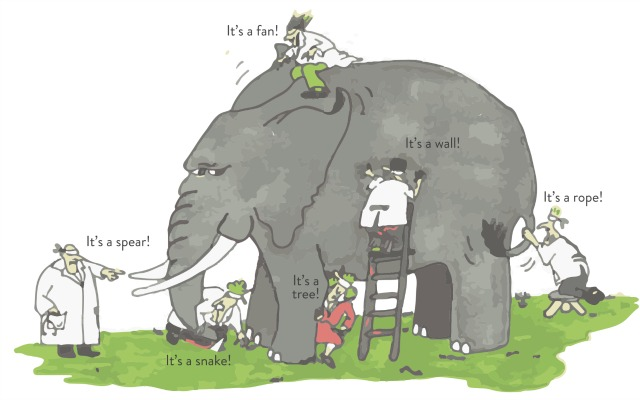
\includegraphics[width=1.2\textwidth]{elephant-and-blinds.jpg}
	\caption{ نگاه محدود و بایاس شده}
\end{figure}

\subsection{تکامل کلان‌داده}
آغاز تکامل کلان‌داده، از سال ۱۹۶۸ بود. اما این امر طی یک یا دو سال محقق نشد. بلکه در دوره‌های زمانی، پیوسته پیشرفت داشت. در ۱۹۶۸ پردازش تراکنش برخط یا \lr{OLTP}، با ظهور تراکنش‌های روزانه در پایگاه‌داده به‌وجود آمد.
در ۱۹۸۳، تکنولوژی انبار داده ظهور پیدا کرد. که این امر به دستاوری به داده‌های تاریخی کمک کرده‌است، که از \lr{OLTP} برای داده‌کاوی استفاده می‌شود.

\subsection{برنامه‌نویسی نگاشت-کاهش}
برنامه‌نویسی نگاشت-کاهش، یک رویکرد جدید برپایه‌ی برنامه‌نویسی شی‌گرا است، که معمولا با زبان جاوا پیاده‌سازی می‌شود. همانطور که از اسم آن پیداست، برنامه به دو قسمت نگاشت و کاهش، تقسیم می‌شود.
همانطور که قبلا اشاره کردیم، هر فایل به چند قسمت تقسیم می‌شود، و هر قسمت برروی یک ماشین، ذخیره می‌شود. در قسمت نگاشت، برنامه برروی تمام ماشین‌های صاحب داده یا \lr{datanode}ها اجرا می‌شود. و داده‌ی برروی ماشین‌را،
به مجموعه‌ای از کلیدها و مقدارها نگاشت می‌کند. برای مثال تمام کلمات موجود در آن بخش فایل‌را در اختیار می‌گیرد، و هرکدام از کلمات‌را به یک کلید و مقدار نگاشت می‌کند، که کلید آن، همان کلمه، و مقدار آن، برابر ۱ است. \\
حال در قسمت کاهش، هرکلید، با تمام مقادیر مقابل آن در اختیار برنامه خواهند بود. و خروجی یک مجموعه از کلیدها و مقدارها است. برای مثال، خروجی نگاشت مرحله‌ی قبل، که شامل کلمه و عدد بود، به صورت کلمه، و لیستی از اعداد، به برنامه داده می‌شود.
حال برنامه با جمع‌کردن، این مقادیر می‌تواند تعداد تکرار آن کلمه، در فایل‌را به‌دست آورد. \\
این رویکرد یک اشکال دارد. و آن این‌است، که در صورتیکه تعداد کلمات زیاد شود، به تعداد تکرار هر کلمه، کلید و مقدار خروجی در مرحله نگاشت، باید از طریق شبکه، به یک ماشین برسد. پس استفاده از شبکه در آن زیاد می‌شود.
پس بهتر است، قبل از ارسال خروجی، به ماشین مقصد، یکبار اعمال کاهش برروی خروجی، اعمال شود، تا استفاده از شبکه بهینه شود. به این کار ترکیب گفته می‌شود.

\begin{figure}[h!]
\centering
        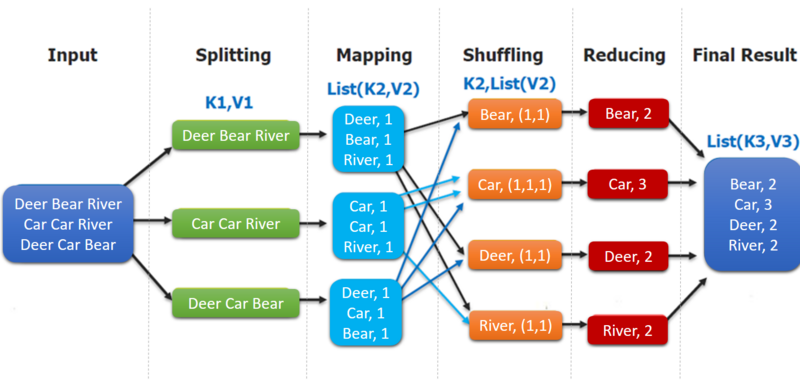
\includegraphics[width=1.0\textwidth]{hadoop-mapreduce.png}
        \caption{مراحل نگاشت کاهش در فریمورک هدوپ}
\end{figure}

\section{کارهای مرتبط}
یادگیری ماشین، افزودن هوش به برنامه است، تا برنامه بتواند یادبگیرد. پروسه‌ی یادگیری به دودسته‌ی یادگیری بانظارت، و بی‌نظارت تقسیم می‌شود. انواع روش‌های یادگیری ماشین در موارد شماره ۱ تا ۶ در منابع یافت می‌شوند.
این تکنیک‌ها در دنیای واقعی نیز مورد استفاده قرار می‌گیرند. \\
همانطور که در منابع و شماره ۷ مشخص‌شده، هدوپ یک فریمورک برنامه‌نویسی به‌صورت توزیع‌شده، است، و با آن می‌توان، مقدار بسیار زیاد داده‌را پردازش کرد.
در هدوپ یک فایل‌سیستم، به‌نام \lr{HDFS} یا \lr{Hadoop Distributed File System} وجود دارد. این فایل‌سیستم به هدوپ امکان مقیاس‌پذیری، می‌دهد. هدوپ می‌تواند با برخی از محصولاتی، که داده‌های خودرا در مموری ذخیره می‌کنند، نیز مقایسه شود.
و حتی از برخی محصولات این دسته، عملکرد بهتری نشان می‌دهد، که در منابع ۸ و ۹ درباره‌ی آن صحبت شده‌است.
سیستم‌های دیگری نیز وجود دارند، که دارای رابط‌های سطح پایین برنامه‌نویسی قدرتمند و متنوع هستند، که در ۱۰ و ۱۱ به آن‌ها اشاره شده است.
مشکل آن‌ها این است که، آن‌ها خاص هستند، و نمی‌توانند رابط سطح بالایی را ارایه دهند.

\section{ فریمورک پیشنهادی برای یادگیری ماشین توزیع‌شده}
ما یک فریمورک یادگیری ماشین، ارایه داده‌ایم، که ماهیتی عمومی دارد، و دارای رابط برنامه‌نویسی سطح بالا می‌باشد. این فریمورک، عملیات رایج برای داده‌های بی‌ساختار را فراهم می‌کند. و در قسمت بکند آن، زمانبندی برای چندکار، به‌صورت همزمان، در محیط توزیع‌شده فراهم می‌کند.
در حقیقت این فریمورک عملیات خوشه‌بندی‌را برای سندها پشتیبانی می‌کند. همینطور \lr{NLP} را نیز ساپورت می‌کند.

\begin{figure}[h!]
    \centering
    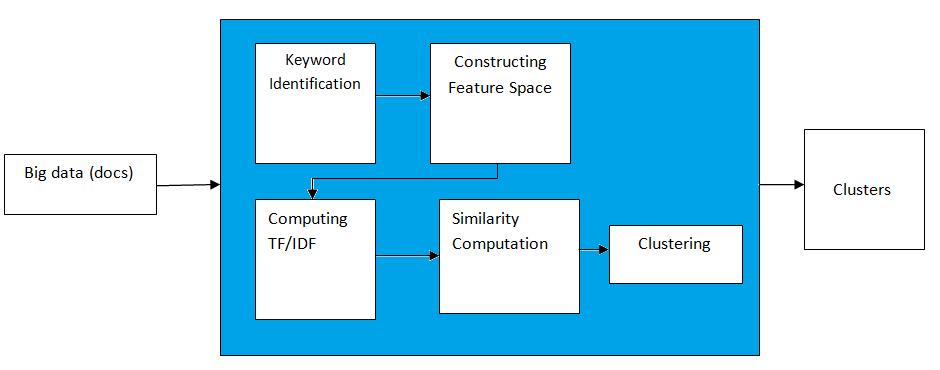
\includegraphics[width=1.2\textwidth]{clustering.png}
    \label{fig:clustering}
    \caption{فریمورک عمومی برای یادگیری ماشین در کلان‌داده}
\end{figure}

در شکل\ref{fig:clustering} کلیات عملیات فریمورک را میبینیم، که اسنادی که باتوجه به مقدار آن‌ها در دسته‌ی کلان‌داده قرار می‌گیرند، را به‌عنوان ورودی گرفته، و خوشه‌ها را خروجی می‌دهد.
در مرحله‌ی اول، کلیدواژه‌ها را پیدا کرده، و سپس \lr{feature}هارا مشحص می‌کند، و مقدار \lr{TF-IDF} آن‌هارا محاسبه می‌کند. سپس الگوریتم محاسبه فاصله‌را مشخص می‌کنیم، و باتوجه به تشابه اسناد، خوشه‌بندی انجام می‌شود.
محاسبه \lr{TF-IDF} به این صورت انجام می‌شود، که دومقدار \lr{term frequency} که برابر تعداد تکرار کلیدواژه، در این سند است، و \lr{document frequency} که تعداد اسنادی است که دارای این کلیدواژه هستند مشخص می‌شود.
سپس ازطریق فرمول زیر مقدار \lr{TF-IDF} مشخص می‌شود.  \\

\begin{equation}
    TF_IDF=TF \times \log \dfrac{N}{DF}
\end{equation}

\begin{figure}[h!]
    \centering
    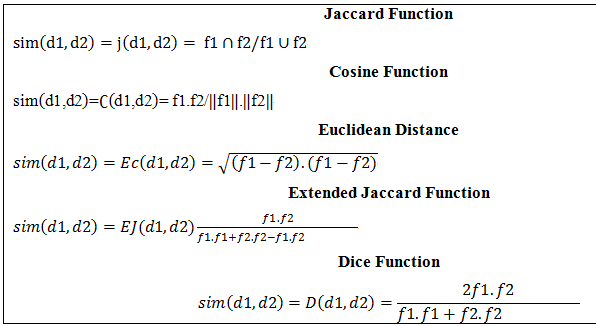
\includegraphics[width=1\textwidth]{distance.png}
    \label{fig:distance}
    \caption{توابع مختلف برای محاسبه‌ی شباهت دوبردار در یادگیری ماشین}
\end{figure}

پس از مشخص شدن بردارها، نوبت به محاسبه‌ی فاصله‌ی میان دوبردار، و درپی آن محاسبه‌ی شباهت میان دوبردار می‌رسد. برای محاسبه‌ی فاصله‌ی میان دوبردار، میتوان از معیارهای اشاره‌شده، در شکل\ref{fig:distance} استفاده کرد.


\section{نتایج تجربی}
ما یک شبیه‌ساز اجرا کردیم که با برنامه‌نویسی توزیع‌شده، مانند هدوپ، و در دوبخش نگاشت و کاهش کار می‌کند. که آن از چند ماشبن، و چند کار همزمان پشتیبانی می‌کند. این فریمورک در پردازش کلان‌داده، و با داده‌های بی‌ساختار مورد آزمون قرار گرفت.
نتایج آن در دوقسمت که یکی \lr{TP} و \lr{FP} بود ارزیابی شد. سیستم دقت ۹۵ درصدی برای \lr{TP} داشت.


\begin{thebibliography}{99}
\bibitem{}
\lr{J. K. Bradley, A. Kyrola, D. Bickson, and C. Guestrin, “Parallel coordinate descent for l1-regularized
loss minimization,” in Proc. Int. Conf. Mach. Learn., 2011, pp. 321–328.}
\bibitem{}
\lr{A. Agarwal and J. C. Duchi, “Distributed delayed stochastic optimization,” in Proc. Adv. Neural Inf.
Process. Syst., 2011, pp. 873–881.}
\bibitem{}
\lr{M. Zinkevich, J. Langford, and A. J. Smola, “Slow learners are fast,” in Proc. Adv. Neural Inf.
Process. Syst., 2009, pp. 2331–2339.}
\bibitem{}
\lr{J. Dean, G. Corrado, R. Monga, K. Chen, M. Devin, Q. Le, M. Mao, M. Ranzato, A. Senior, P.
Tucker, K. Yang, and A. Ng, “Large scale distributed deep networks,” in Proc. Adv. Neural Inf.
Process. Syst., 2012, pp. 1232–1240.}
\bibitem{}
\lr{M. D. Hoffman, D. M. Blei, C. Wang, and J. Paisley, “Stochastic variational inference,” J. Mach.
Learn. Res., vol. 14, pp. 1303–1347, 2013.}
\bibitem{}
\lr{S. A. Williamson, A. Dubey, and E. P. Xing, “Parallel Markov chain Monte Carlo for nonparametric
mixture models,” in Proc.Int. Conf. Mach. Learn., 2013, pp. 98–106.}
\bibitem{}
\lr{T. White, Hadoop: The Definitive Guide. Sebastopol, CA, USA: O’Reilly Media, 2012}
\bibitem{}
\lr{Y. Low, J. Gonzalez, A. Kyrola, D. Bickson, C. Guestrin, and J. M. Hellerstein, “Distributed
GraphLab: A framework for machine learning and data mining in the cloud,” in Proc. VLDB
Endowment, vol. 5, pp. 716–727, 2012.}
\bibitem{}
\lr{M. Zaharia, M. Chowdhury, M. J. Franklin, S. Shenker, and I. Stoica, “Spark: Cluster computing with
working sets,” in Proc. 2nd USENIX Conf. Hot Topics Cloud Comput., 2010, p. 10.}
\bibitem{}
\lr{M. Li, D. G. Andersen, J. W. Park, A. J. Smola, A. Ahmed, V. Josifovski, J. Long, E. J. Shekita, and
B.-Y. Su, “Scaling distributed machine learning with the parameter server,” in Proc. 11th USENIX
Conf. Operating Syst. Des. Implementation, 2014, pp. 583–598.}
\bibitem{}
\lr{R. Power and J. Li, “Piccolo: Building fast, distributed programs with partitioned tables,” in Proc.
USENIX Conf. Operating Syst. Des. Implementation, article 10, 2010, pp. 1–14.}
\end{thebibliography}
\end{document}
